% This file was created by tikzplotlib v0.9.8.
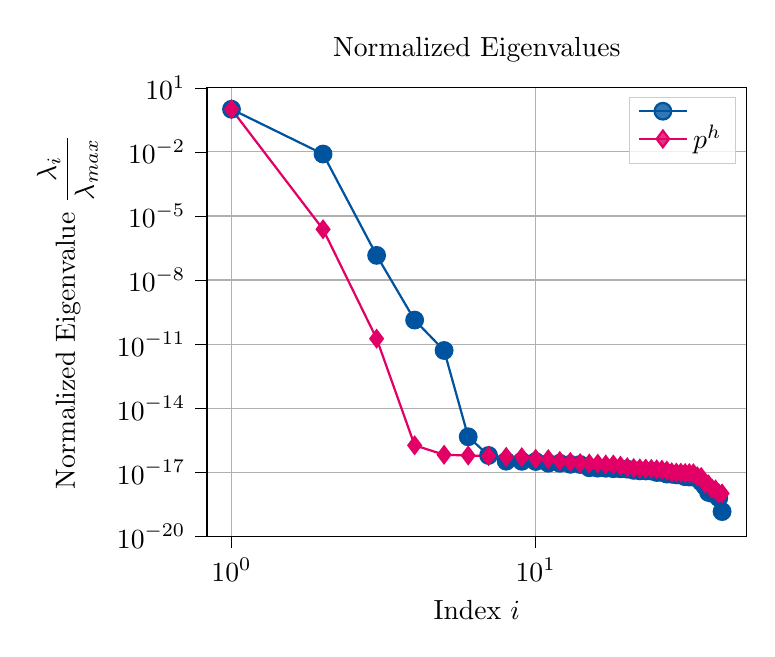
\begin{tikzpicture}

\definecolor{color0}{rgb}{0,0.329411764705882,0.623529411764706}
\definecolor{color1}{rgb}{0.890196078431372,0,0.4}

\begin{axis}[
legend cell align={left},
legend style={fill opacity=0.8, draw opacity=1, text opacity=1, draw=white!80!black},
log basis x={10},
log basis y={10},
tick align=outside,
tick pos=left,
title={Normalized Eigenvalues},
x grid style={white!69.0196078431373!black},
xlabel={Index \(\displaystyle i\)},
xmajorgrids,
xmin=0.830540485032707, xmax=49.3654442364545,
xmode=log,
xtick style={color=black},
xtick={0.01,0.1,1,10,100,1000},
xticklabels={
  \(\displaystyle 10^{-2}\),
  \(\displaystyle 10^{-1}\),
  \(\displaystyle 10^{0}\),
  \(\displaystyle 10^{1}\),
  \(\displaystyle 10^{2}\),
  \(\displaystyle 10^{3}\)
},
y grid style={white!69.0196078431373!black},
ylabel={Normalized Eigenvalue \(\displaystyle \frac{\lambda_i}{\lambda_{\text{max}}}\)},
ymajorgrids,
ymin=1e-20, ymax=10,
ymode=log,
ytick style={color=black},
ytick={1e-23,1e-20,1e-17,1e-14,1e-11,1e-08,1e-05,0.01,10,10000},
yticklabels={
  \(\displaystyle 10^{-23}\),
  \(\displaystyle 10^{-20}\),
  \(\displaystyle 10^{-17}\),
  \(\displaystyle 10^{-14}\),
  \(\displaystyle 10^{-11}\),
  \(\displaystyle 10^{-8}\),
  \(\displaystyle 10^{-5}\),
  \(\displaystyle 10^{-2}\),
  \(\displaystyle 10^{1}\),
  \(\displaystyle 10^{4}\)
}
]
\addplot [thick, color0, mark=*, mark size=3, mark options={solid}]
table {%
1 1
2 0.00794975858415845
3 1.42582257382325e-07
4 1.32791974403868e-10
5 5.00366283890635e-12
6 4.54114155240754e-16
7 6.04573529497411e-17
8 3.26201133022688e-17
9 3.22574638852698e-17
10 3.15358446366046e-17
11 2.62454621731955e-17
12 2.60840954654917e-17
13 2.33242093571454e-17
14 2.28813585566599e-17
15 1.60218882337199e-17
16 1.54306862706516e-17
17 1.52807821353466e-17
18 1.44864745846082e-17
19 1.43851705211444e-17
20 1.38677194525787e-17
21 1.21734236816605e-17
22 1.14897279038485e-17
23 1.13956935268721e-17
24 1.12564920102658e-17
25 9.63808041350083e-18
26 9.58979066065725e-18
27 8.13046505587439e-18
28 8.00740202533402e-18
29 7.46188080562777e-18
30 7.26718042554605e-18
31 6.11314351785897e-18
32 5.93273799548898e-18
33 5.84970067761768e-18
34 5.29939613242502e-18
35 3.47549460184894e-18
36 2.1905261247255e-18
37 1.12228744856004e-18
38 1.01406198292573e-18
39 9.59373162820783e-19
40 6.26226288149959e-19
41 1.42523827201686e-19
};
\addlegendentry{$\trialVelocityHomDiscrete$}
\addplot [thick, color1, mark=diamond*, mark size=3, mark options={solid}]
table {%
1 1
2 2.37328846603967e-06
3 1.78817929292869e-11
4 1.81154657334976e-16
5 6.51678466039161e-17
6 6.02235881107004e-17
7 5.69247083103718e-17
8 5.20065737906182e-17
9 5.01348143603465e-17
10 4.20958043774671e-17
11 4.07622974109276e-17
12 3.32697934377648e-17
13 2.98511733192585e-17
14 2.64421964531683e-17
15 2.52583071694472e-17
16 2.48386648445979e-17
17 2.27569426656641e-17
18 2.27247846357554e-17
19 1.99821382141988e-17
20 1.70491132142761e-17
21 1.54624364513944e-17
22 1.49112670601225e-17
23 1.45406520529215e-17
24 1.40935012359226e-17
25 1.35426769923973e-17
26 1.2976308799412e-17
27 1.18179500955933e-17
28 9.80114361457536e-18
29 9.51423374282225e-18
30 9.36239599182889e-18
31 9.08584610553105e-18
32 8.96571848518543e-18
33 8.78366822577326e-18
34 6.40001828288954e-18
35 5.93546015704658e-18
36 2.97856912325833e-18
37 2.64216217074413e-18
38 1.67829393129063e-18
39 1.53977850304594e-18
40 1.02797999983454e-18
41 1.00473640799576e-18
};
\addlegendentry{$p^h$}
\end{axis}

\end{tikzpicture}
